\input ../SlidePreamble
\input ../preamble

\begin{document}

{\Huge

  \centerline{\bf TTIC 31230, Fundamentals of Deep Learning}
  \bigskip
  \centerline{David McAllester, Winter 2019}
  \vfill
  \centerline{Controlling Gradients}
  \vfill
  \vfill
  \centerline{Vanishing and Exploding Gradients}
  \vfill
  \centerline{Initialization}
  \vfill
  \centerline{Batch Normalization}
  \vfill
  \centerline{Residual Networks}
  \vfill
  \centerline{Gated RNNs}

\slide{Vanishing and Exploding Gradients}
~
\vfill
\centerline{Causes of Vanishing and Exploding Gradients:}
\vfill
\centerline{Activation function saturation}
\vfill
\centerline{Repeated multiplication by network weights}
\vfill

\slide{Activation Function Saturation}

Consider the sigmoid activation function $1/(1+ e^{-x})$.

\vfill
\centerline{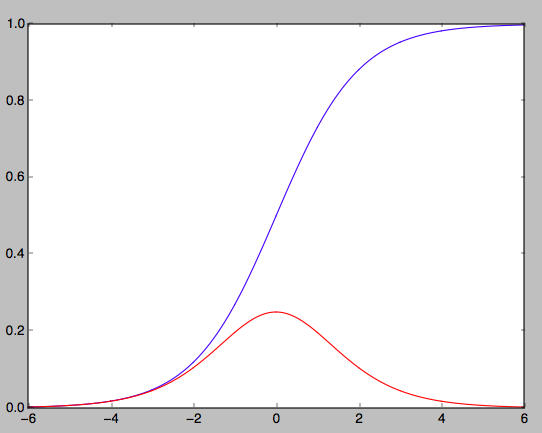
\includegraphics[width= 4.0in]{../images/sigmoid2}}


\vfill
The gradient of this function is quite small for $|x| > 4$.

\vfill
In deep networks backpropagation can go through many sigmoids and
the gradient can ``vanish''

\slide{Activation Function Saturation}

$\mathrm{Relu}(x) = \max(x,0)$

\vfill
\centerline{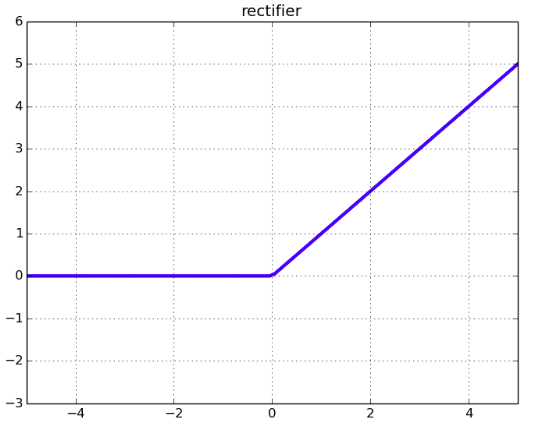
\includegraphics[width= 4.0in]{../images/relu}}

\vfill
The Relu does not saturate at positive inputs (good) but is completely saturated at negative inputs (bad).

\vfill
Alternate variations of Relu still have small gradients at negative inputs.

\slide{Repeated Multiplication by Network Weights}

Consider a deep CNN.

$$L_{i+1} = \mathrm{Relu}(\mathrm{Conv}(\Phi_i,L_i))$$

\vfill
For $i$ large, $L_i$ has been multiplied by many weights.

\vfill
If the weights are small then the neuron values, and hence the weight gradients, decrease exponentially with depth. {\bf Vanishing Gradients.}

\vfill
If the weights are large, and the activation functions do not saturate, then the neuron values, and hence the weight gradients,
increase exponentially with depth. {\bf Exploding Gradients.}

\slide{Methods for Maintaining Gradients}

\centerline{Initialization}

\vfill
\centerline{Batch Normalization}

\vfill
\centerline{Highway Architectures (Skip Connections)}

\slide{Methods for Maintaining Gradients}

\centerline{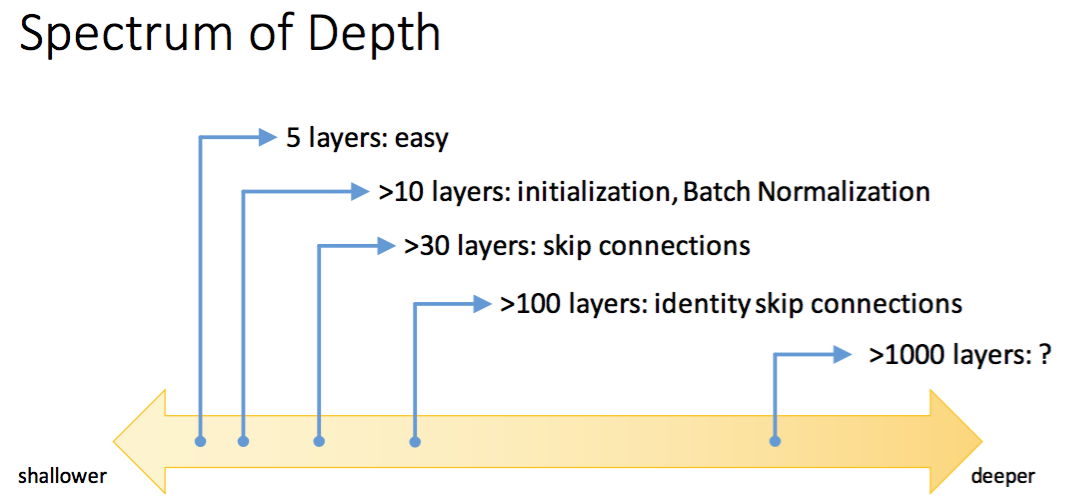
\includegraphics[width = 9in]{../images/DepthSpectrum}}

\centerline{\large Kaiming He}

\slide{}
\centerline{\bf Initialization}
\vfill

\slide{Xavier Initialization}

Initialize a weight matrix (or tensor) to preserve zero-mean unit variance distributions.

\vfill
If we assume $x_i$ has unit mean and zero variance then we want

\vfill
$$y_j = \sum_{j=0}^{N-1} x_i w_{i,j}$$

\vfill
to have zero mean and unit variance.

\vfill
Xavier initialization randomly sets $w_{i,j}$ to be uniform in the interval $\left(-\sqrt{\frac{3}{N}},\;\sqrt{\frac{3}{N}}\right)$.

\vfill
Assuming independence this gives zero mean and unit variance for $y_j$.

\slide{He Initialization}

A Relu nonlinearity reduces the variance.

\vfill
Before a Relu nonlinearity it seems better to use the larger interval $\left(-\sqrt{\frac{6}{N}},\;\sqrt{\frac{6}{N}}\right)$.

\slide{}
\centerline{\bf Batch Normalization}
\vfill

\slide{Normalization}
Given a tensor $x[b,j]$ we define $\tilde{x}[b,j]$ as follows.

\begin{eqnarray*}
  \hat{\mu}[j] & = & \frac{1}{B} \sum_b\;x[b,j] \\
  \\
  \\
  \hat{\sigma}[j] & = & \sqrt{\frac{1}{B-1} \sum_b (x[b,j]-\hat{\mu}[j])^2} \\
  \\
  \\
  \tilde{x}[b,j]& = & \frac{x[b,j] - \hat{\mu}[j]}{\hat{\sigma}[j]}
\end{eqnarray*}


\vfill
At test time a single fixed estimate of $\mu[j]$ and $\sigma[j]$ is used.

\slide{Spatial Batch Normalization}

For CNNs we convert a tensor $x[b,x,y,j]$ to $\tilde{x}[b,x,y,j]$ as follows.

\begin{eqnarray*}
  \hat{\mu}[j] & = & \frac{1}{BXY} \sum_{b,x,y}\;x[b,x,y,j] \\
  \\
  \\
  \hat{\sigma}[j] & = & \sqrt{\frac{1}{BXY-1} \sum_{b,x,y} (x[b,x,y,j]-\hat{\mu}[j])^2} \\
  \\
  \\
  \tilde{x}[b,x,y,j]& = & \frac{x[b,x,y,j] - \hat{\mu}[j]}{\hat{\sigma}[j]}
\end{eqnarray*}

\slide{Adding an Affine Transformation}

$$\breve{x}[b,x,y,j] = \gamma[j] \tilde{x}[b,x,y,j] + \beta[j]$$

\vfill
Here $\gamma[j]$ and $\beta[j]$ are parameters of the batch normalization.

\vfill
This allows the batch normlization to learn an arbitrary affine transformation (offset and scaling).

\vfill
It can even undo the normaliztion.

\slide{Batch Normalization}

Batch Normalization appears to be generally useful in CNNs but is not always used.

\vfill
Not so successful in RNNs.

\vfill
It is typically used just prior to a nonlinear activation function.

\vfill
It is intuitively justified in terms of ``internal covariate shift'':
as the inputs to a layer change the zero mean unit variance property underlying Xavier initialization are maintained.

\ignore{
\slide{Normalization Interacts with SGD}

Consider backpropagation through a weight layer.

\begin{eqnarray*}
  y.\mathrm{value}[\cdots] & \pluseq & w.\mathrm{value}[\cdots]\;x.\mathrm{value}[\dots] \\
  \\
  \\
  w.\mathrm{grad}[\cdots] & \pluseq & y.\mathrm{grad}[\cdots]\;x.\mathrm{value}[\cdots]
\end{eqnarray*}

\vfill
Replacing $x$ by $x/\hat{\sigma}$ seems related to RMSProp for the update of $w$.

\slide{The Simple Normalization Conjecture}

A simple normalization layer $y = \alpha (x + \beta)$ can be used in place of batch normalization as long $\beta$ is initialized to $-\hat{\mu}$
and $\alpha$ is initialized to $1/\hat{\sigma}$.

\vfill
Here $\hat{\mu}$ and $\hat{\sigma}$ should be computed only after earlier normalizations have been properly initialized.
}

\vfill
\eject
~ \vfill
\centerline{\bf Highway Architectures (Skip Connections)}
\vfill
\vfill

\slide{Deep Residual Networks (ResNets) by Kaiming He 2015}

\vfill
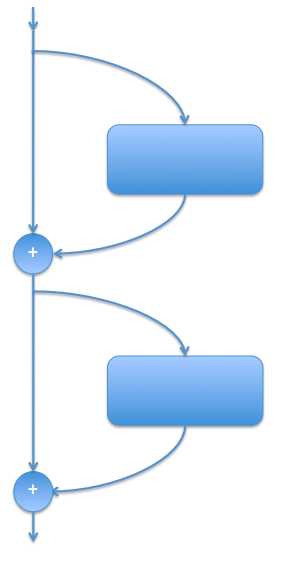
\includegraphics[width= 2.5in]{../images/resnet}
\hfill \begin{minipage}[b]{4in}
  A ``skip connection'' is adjusted by a ``residual correction''

  \bigskip
  The skip connections connects input to output directly and hence preserves gradients.

  \bigskip
  ResNets were introduced in late 2015 (Kaiming He et al.) and revolutionized computer vision.
\end{minipage}

\slideplain{Simple Residual Skip Connections in CNNs (stride 1)}

$$L_{i+1} = L_i + R_i$$

\vfill
In ResNet $R_i$ is computed by two or three convolution layers.

\vfill
If all convolution layers are stride 1, and preserve the number of channels, then $R_i$ and $L_i$ are the same shape.

\slideplain{Handling Spacial Reduction}

Let the shape of $L_i$ be $[B,X_i,Y_i,J_i]$.

\vfill
Let the shape of $R_i$ be $[B,X_{i+1},Y_{i+1},J_{i+1}]$ where $X_{i+1} = X_i/s$ and $Y_{i+1} = Y_i/s$ for some stride $s$, and where $J_{i+1} \geq J_i$.

\vfill
In this case we construct $\tilde{L}_i$ to have the same shape as $R_i$.

\vfill
\begin{eqnarray*}
\tilde{L}_i[b,x,y,j] & = & \left\{\begin{array}{ll} L_i[b,s*x,s*y,j] & \mbox{for $j < J_i$} \\ 0 & \mbox{otherwise} \end{array}\right.\\
\\
L_{i+1} & = & \tilde{L}_i  + R_i
\end{eqnarray*}

\slide{Resnet32}

\centerline{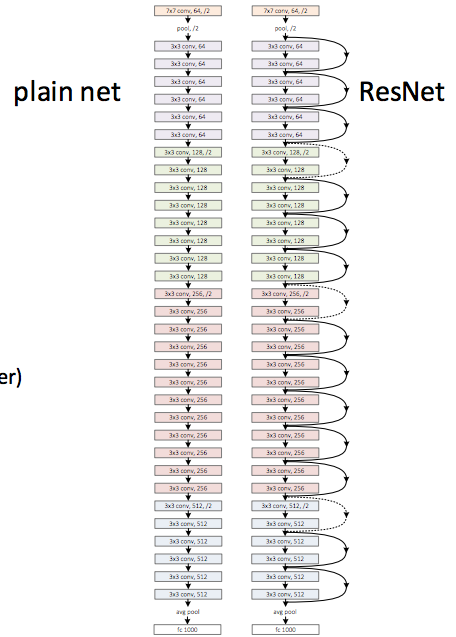
\includegraphics[height= 5.5in]{../images/ResnetStack} {\large [Kaiming He]}}


\slideplain{Deeper Versions use Bottleneck Residual Paths}
We reduce the number of channels to $K < J_i$ before doing the convolution.

{\huge
\begin{eqnarray*}
A_i[B,X_i,Y_i,K] & = & \mathrm{Conv}'(\Phi_i^A{\color{red} [1,1,J_i,K]},L_i[B,X_i,Y_i,J_i]) \\
\\
B_i[B,X_{i+1},Y_{i+1},K] & = & \mathrm{Conv}'(\Phi_i^B{\color{red}[3,3,K,K]},A_i[B,X_i,Y_i,K],\;\mathrm{stride}\;s) \\
\\
R_i[B,X_{i+1},Y_{i+1},J_{i+1}] & = & \mathrm{Conv}'(\Phi_i^R{\color{red} [1,1,K,J_{i+1}]},B_i[B,X_{i+1},Y_{i+1},K]) \\
\\
L_{i+1} & = & \tilde{L}_i + R_i
\end{eqnarray*}
}

\vfill
Here $\mathrm{CONV}'$ may include batch normalization and/or an activation function.

\slideplain{Deep Residual Networks}

\vfill
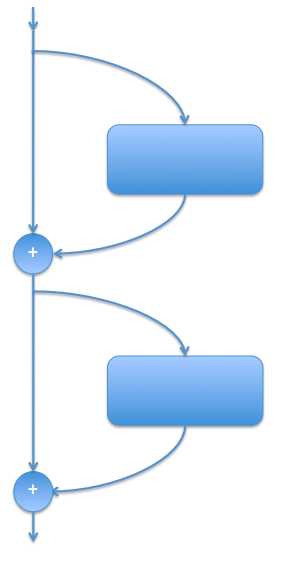
\includegraphics[width= 2.5in]{../images/resnet}
\hfill \begin{minipage}[b]{4in} As with most of deep learning, not much is known about what resnets are actually doing.
  
  \bigskip
  \bigskip
  For example, different residual paths might update disjoint channels making the networks shallower than they look.

  \bigskip
  \bigskip
  They are capable of representing very general circuit topologies.
\end{minipage}

\slideplain{}
\vfill
\centerline{Recurrent Neural Networks (RNNs)}
\vfill
\vfill

\slide{Vanilla RNNs}



\centerline{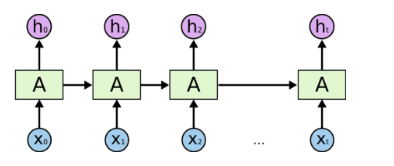
\includegraphics[width=3.5in]{../images/RNN}}
\centerline{{\large [Christopher Olah]}}

$$\tilde{h}_{t+1}[b,j] = \left(\sum_i\;W^{h,h}[i,j]h_t[b,i]\right) + \left(\sum_k W^{x,h}[k,j]x_t[b,k]\right) + \beta[j]$$

\vfill
$$\mathrm{Parameter}\;\Phi = (W^{h,h}[J,J],\;W^{x,h}[K,J],\;\beta[J])$$

\slideplain{Exploding and Vanishing Gradients}

An RNN uses the same weights at every time step.

\vfill
If we avoid saturation of the activation functions then we get exponentially growing or shrinking eigenvectors of the weight matrix.

\vfill
Note that if the forward values are bounded by sigmoids or tanh then they cannot explode.

\vfill
However the gradients can still explode.

\slide{Exploding Gradients: Gradient Clipping}

\vfill
We can dampen the effect of exploding gradients by clipping them before applying SGD.

\vfill
$$W.\mathrm{grad} = \left\{\begin{array}{l} W.\mathrm{grad} \;\;\;\mbox{if $||W.\mathrm{grad}|| \leq n_{\mathrm{max}}$} \\
                                                      \\ \\
                                                      n_{\mathrm{max}} \; W.\mathrm{grad} / ||W.\mathrm{grad}|| \;\; \mbox{otherwise}
\end{array} \right.$$

\vfill
See {\tt torch.nn.utils.clip\_grad\_norm}

\slide{Vanishing Gradients: Gated Skip Connections}


$$\begin{array}{lrcl}
\mbox{Residual Skip:} & L_{i+1} & = & \tilde{L}_i + R_i \\
\mbox{(layer-specific parameters)} \\
\\
\\
\mbox{Gated Skip:} & h_{t+1} & = & G_t\odot h_t + (1-G_t)\odot R_t \\
\mbox{(time-independent parameters)}
\end{array}$$

\vfill
\begin{eqnarray*}
(G\odot h)[b,j] & = & G[b,j] * h[b,j] \\
\\
(1-G_t)[b,j] & = & 1-G_t[b,j]
\end{eqnarray*}

\vfill
Gating allows data dependent data flow.

\slideplain{Update Gate RNN (UGRNN)}

{\huge
\begin{eqnarray*}
\tilde{R}_t[b,j] & = & \left(\sum_i\;W^{h,R}[i,j]h_t[b,i]\right) + \left(\sum_k W^{x,R}[k,j]x_t[b,k]\right) + \beta^R[j] \\
\\
\\
\tilde{G}_t[b,j] & = & \left(\sum_i\;W^{h,G}[i,j]h_t[b,i]\right) + \left(\sum_k W^{x,G}[k,j]x_t[b,k]\right) + \beta^G[j] \\
\\
\\
h_{t+1}[b,j] & = & \sigma(G_t[b,j]) h_t[b,j] + (1-\sigma(G_t[b,j])) \tanh(R_t[b,j]) \\
\\
\\
\Phi & = & (W^{h,R},W^{x,R},\beta^R,W^{h,G},W^{x,G},\beta^G)
\end{eqnarray*}
}

\slide{Gated Recurrent Unity (GRU) by Cho et al. 2014}

\centerline{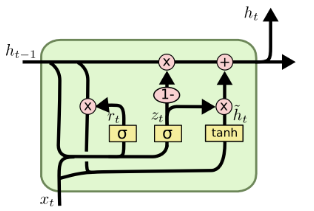
\includegraphics[width=6.0in]{../images/GRU}}
\centerline{{\huge [Christopher Olah]}}

\slide{Long Short Term Memory (LSTM)}
\centerline{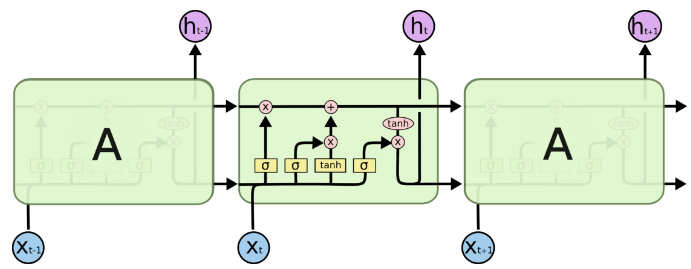
\includegraphics[width=3.5in]{../images/LSTM}}
\centerline{{\large [figure: Christopher Olah]}}

\centerline{\Large [LSTM: Hochreiter\&Shmidhuber, 1997]}

\slide{UGRNN vs. GRUs vs. LSTMs}

\vfill
In class projects from previous years, GRUs consistently outperformed LSTMs.

\vfill
A systematic study [Collins, Dickstein and Sussulo 2016] states:

\begin{quotation}
  Our results point to the GRU as being the most learnable of gated RNNs for shallow architectures, followed by the UGRNN.
\end{quotation}

\slideplain{END}

}
\end{document}
